\chapter{Principes de base}
\label{chap:bases}

\section{Rédaction}
\label{chap:bases:redaction}

Lors de l'apprentissage de {\LaTeX} la personne habituée à utiliser un
traitement de texte  devra fort probablement se défaire d'une vilaine
habitude: se préoccuper sans cesse de la disposition et de l'apparence
du texte au moment de la rédaction.

En effet, avec un système de mise en page tel que {\LaTeX}, on se
concentre sur le contenu et la \emph{structure} du document à la
rédaction, et non pas sur son \emph{apparence}. Par exemple:
\begin{itemize}
\item au lieu de prescrire qu'un titre de section doit être en gras
  14~points, on indique simplement à {\LaTeX} que le texte doit être
  traité comme un titre de section
  \begin{demo}
    \begin{minipage}{0.45\linewidth}
\begin{lstlisting}
\textbf{\large Titre}
\end{lstlisting}
    \end{minipage}
    \hfill \faArrowRight \hfill
    \begin{minipage}{0.45\linewidth}
\begin{lstlisting}
\section{Titre}
\end{lstlisting}
    \end{minipage}
  \end{demo}
\item au lieu de décider qu'un mot sur lequel l'on souhaite insister
  sera en italique, on indique à {\LaTeX} de mettre de l'emphase sur
  ce mot sans se soucier de la mise en forme
  \begin{demo}
    \begin{minipage}{0.45\linewidth}
\begin{lstlisting}
\textit{texte}
\end{lstlisting}
    \end{minipage}
    \hfill \faArrowRight \hfill
    \begin{minipage}{0.45\linewidth}
\begin{lstlisting}
\emph{texte}
\end{lstlisting}
    \end{minipage}
  \end{demo}
\end{itemize}

L'apparence du texte sera prise en charge par {\LaTeX}. Comme les
gabarits sont l'{\oe}uvre de spécialistes en typographie, il est
généralement préférable de ne pas les modifier. À titre d'exemple,
{\LaTeX} détermine automatiquement la largeur des marges en fonction
de la taille de la police de caractère de manière à ce que les lignes
de texte ne dépassent pas approximativement 70~caractères. La raison:
lorsqu'une ligne de texte est trop longue, notre {\oe}il a de la
difficulté à la suivre sur toute sa longueur. Il a tendance à passer à
la ligne inférieure, ce qui rend la lecture plus difficile.

Une fois ce principe de séparation du contenu et de l'apparence
compris et accepté, on veillera, lors de la saisie du texte, à
respecter les règles simples suivantes.
\begin{enumerate}
\item On sépare les mots par une ou plusieurs \emph{espaces}. Qu'il y
  en ait une ou un millier, seule la première compte et la mise en
  page sera la même.
  \begin{demo}
    \begin{texample}
\begin{lstlisting}[showspaces=true]
Les espaces délimitent les
mots. Leur nombre n'a pas
d'importance.
\end{lstlisting}
      \producing
      Les espaces délimitent les
      mots. Leur nombre n'a pas
      d'importance.
    \end{texample}
    \begin{texample}
\begin{lstlisting}[showstringspaces=true]
Les  espaces   délimitent
les                 mots.
Leur    nombre  n'a pas
d'importance.
\end{lstlisting}
      \producing
      Les  espaces   délimitent
      les                 mots.
      Leur    nombre  n'a pas
      d'importance.
    \end{texample}
  \end{demo}
%
\item On sépare les paragraphes par une ou plusieurs lignes blanches.
  Celles-ci n'apparaîtront pas nécessairement dans le texte final; les
  gabarits standards identifient les paragraphes par un retrait de
  première ligne.
  \begin{demo}
    \begin{texample}
\begin{lstlisting}
Les lignes blanches
délimitent les
paragraphes.

Leur nombre n'a pas
d'importance.
\end{lstlisting}
      \producing
Les lignes blanches
délimitent les
paragraphes.

        Leur nombre n'a pas
        d'importance.
    \end{texample}
\begin{texample}
\begin{lstlisting}
Les lignes blanches
délimitent les
paragraphes.



Leur nombre n'a pas
d'importance.
\end{lstlisting}
      \producing
        Les lignes blanches  délimitent
        les paragraphes.



        Leur nombre n'a pas
        d'importance.
    \end{texample}
  \end{demo}
%
\item On utilise des \emph{commandes} pour indiquer la structure du
  texte dans le code source.
\end{enumerate}


\section{Structure d'un document}
\label{chap:bases:structure}

Un fichier source {\LaTeX} --- dont on trouvera un exemple simple à la
\autoref{fig:bases:parties} --- est toujours composé de deux parties.

\begin{figure}
  \centering
  \begin{minipage}{0.75\linewidth}
\begin{lstlisting}[numbers=left, numberstyle=\tiny]
\documentclass[11pt,french]{article} `\label{lst:bases:preambule_debut}'
  \usepackage{babel}
  \usepackage[autolanguage]{numprint}
  \usepackage[utf8]{inputenc}
  \usepackage[T1]{fontenc} `\label{lst:bases:preambule_fin}'

\begin{document} `\label{lst:bases:corps_debut}'

Lorem ipsum dolor sit amet, consectetur
adipiscing elit. Donec quam nulla, bibendum
vitae ipsum vel, fermentum pellentesque orci.

\end{document} `\label{lst:bases:corps_fin}'
\end{lstlisting}
  \end{minipage}
  \caption{Fichier source {\LaTeX} simple comportant les deux parties
    obligatoires: le préambule (lignes
    \ref*{lst:bases:preambule_debut}--\ref*{lst:bases:preambule_fin})
    et le corps du document (lignes
    \ref*{lst:bases:corps_debut}--\ref*{lst:bases:corps_fin}).}
  \label{fig:bases:parties}
\end{figure}

\begin{description}
\item[Préambule] Suite de commandes spécifiant la mise en forme
  globale du document (format du papier, marges, entête et pied de
  page, etc.). Il contient au minimum la commande
  \cmd{\documentclass}. Les commandes contenues dans le préambule ont
  un effet global sur le document.

  Dans l'exemple de la \autoref{fig:bases:parties}, le préambule
  s'étend de la ligne \ref*{lst:bases:preambule_debut} à la ligne
  \ref*{lst:bases:preambule_fin}.
\item[Corps du document] Contenu du document en tant que tel.
  Il débute par \verb=\begin{document}= et se termine par
    \verb=\end{document}=. Le corps du document peut aussi contenir
  des commandes, mais l'effet de celles-ci est presque toujours local.

  Les lignes \ref*{lst:bases:corps_debut}--\ref*{lst:bases:corps_fin}
  du code de la \autoref{fig:bases:parties} forment le corps de ce
  document.
\end{description}


\section{Commandes}
\label{chap:bases:commandes}

{\LaTeX} étant un langage de programmation servant à indiquer la
disposition du texte sur une page par le biais de commandes, il
convient d'étudier la syntaxe du langage afin de pouvoir l'utiliser.
Cette courte section se penche spécifiquement sur la syntaxe des
commandes.

Les formes générales des commandes {\LaTeX} sont:
\begin{lstlisting}
\`\meta{nomcommande}\oarg{arg\_optionnel}\marg{arg\_obligatoire}'
\`\meta{nomcommande}'*`\oarg{arg\_optionnel}\marg{arg\_obligatoire}'
\end{lstlisting}
Ici, \meta{nomcommande} est le nom de la commande. Il débute par le
caractère {\bs} et est exclusivement formé de lettres, habituellement
des minuscules ({\LaTeX} est sensible à la casse). Lorsque la commande
prend des arguments, les arguments obligatoires sont placés entre
accolades \verb={ }= et les arguments optionnels sont placés entre
crochets \verb=[ ]=.

Certaines commandes n'ont aucun argument. Leur forme est alors
\begin{lstlisting}
\`\meta{nomcommande}
\end{lstlisting}
Dans ce cas, le nom d'une commande se termine par tout caractère qui
n'est pas une lettre --- y compris l'espace! Cette règle fait en sorte
qu'une espace après le nom d'une commande est considéré comme un
marqueur de la fin du nom de celle-ci. Cette règle joue parfois de
vilains tours en «avalant» l'espace entre une commande et le mot qui
suit; voir l'\autoref{exemple:base:commandes} et
l'\autoref{ex:base:commandes}.

La forme étoilée d'une commande réalise généralement une action
légèrement différente de la version sans étoile. Par exemple, la
commande \cmd{\section} crée une nouvelle section numérotée, alors que
\cmd{\section*} n'insère aucune numérotation.

La portée d'une commande est limitée à la zone entre accolades
\verb={ }=, le cas échéant.

\begin{exemple}
  \label{exemple:base:commandes}
  Voici trois exemples de commandes {\LaTeX}: une sans argument, une
  avec un seul argument obligatoire et une commande avec deux
  arguments obligatoires et un argument optionnel.
  \begin{enumerate}
  \item La commande \cmd{\LaTeX} permet de composer de logo {\LaTeX}.
    \begin{demo}
      \begin{texample}
\begin{lstlisting}
Apprendre \LaTeX c'est
formidable!
\end{lstlisting}
        \producing
        Apprendre \LaTeX c'est
        formidable!
      \end{texample}
    \end{demo}
    On constate ici l'effet de la règle mentionnée précédemment:
    l'espace suivant le nom de la commande a été interprété par
    {\LaTeX} comme un marqueur de la fin de la commande et il a été
    supprimé du texte. Pour contourner ce problème, nous pouvons soit
    fournir un argument vide à la commande, soit la placer en
    accolades pour limiter sa portée à elle-même:
    \begin{demo}
      \begin{texample}
\begin{lstlisting}
Apprendre \LaTeX{} c'est
formidable!
\end{lstlisting}
        \producing
        Apprendre \LaTeX{} c'est
        formidable!
      \end{texample}
      \begin{texample}
\begin{lstlisting}
Apprendre {\LaTeX} c'est
formidable!
\end{lstlisting}
        \producing
        Apprendre {\LaTeX} c'est
        formidable!
      \end{texample}
    \end{demo}
    %
  \item La commande \cmd{\emph} met de l'emphase (en général sous
    forme d'italique) sur le ou les mots en argument.
    \begin{demo}
      \begin{texample}
\begin{lstlisting}
Il est \emph{essentiel} de
connaître la syntaxe de
{\LaTeX}.
\end{lstlisting}
        \producing
        Il est \emph{essentiel} de
        connaître la syntaxe de
        {\LaTeX}.
      \end{texample}
    \end{demo}
    %
  \item La commande \cmd{\rule} produit un rectangle plein. Elle a
    deux arugments obligatoires: la longueur et la hauteur du
    rectangle, dans l'ordre. Un argument optionnel permet de surélever
    le rectangle au-dessus de la ligne de base (voir le
    \autoref{chap:boites} pour plus de détails).
    \begin{demo}
      \begin{texample}
\begin{lstlisting}
Réglure de 1~cm de long et
3~mm d'épais surélevée de
2~points au-dessus de la
ligne de base:
\rule[2pt]{1cm}{3mm}.
\end{lstlisting}
        \producing
        Réglure de $1$~cm de long et
        $3$~mm d'épais surélevée de
        $2$~points au-dessus de la
        ligne de base: \rule[2pt]{1cm}{3mm}.
      \end{texample}
    \end{demo}
  \end{enumerate}
  \qed
\end{exemple}

\begin{exemple}
  La commande \cmd{\bfseries} sélectionne une police de caractère
  grasse pour tout le texte qui suit.
  \begin{demo}
    \begin{texample}
\begin{lstlisting}
En typographie, la \bfseries
graisse est l'épaisseur d'un
trait ou d'un caractère.
\end{lstlisting}
      \producing
      En typographie, la \bfseries
      graisse est l'épaisseur d'un
      trait ou d'un caractère.
    \end{texample}
  \end{demo}
  Pour limiter le changement à une zone de texte, il faut la délimiter
  par des accolades.
\begin{demo}
    \begin{texample}
\begin{lstlisting}
En typographie, la {\bfseries
graisse est l'épaisseur d'un
trait} ou d'un caractère.
\end{lstlisting}
      \producing
      En typographie, la {\bfseries
      graisse est l'épaisseur d’un
      trait} ou d’un caractère.
    \end{texample}
  \end{demo}
  \qed
\end{exemple}

L'usager de {\LaTeX} peut définir de nouvelles commandes à loisir, tel
qu'expliqué à la \autoref{sec:commandes:commandes}.


\section{Environnements}
\label{chap:bases:environnements}

Un environnement {\LaTeX} est simplement une zone de texte délimitée
une construction du type
\begin{lstlisting}
\begin`\marg{environnement}'
   ...
\end`\marg{environnement}'
\end{lstlisting}
Le contenu d'un environnement est traité différemment du reste du
texte en fonction des paramètres de l'environnement. Par exemple, le
texte à l'intérieur d'un environnement \Ie{center} est centré sur la
page.

Les changements induits par un environnement s'appliquent uniquement à
l'intérieur de celui-ci. Il en va de même des commandes utilisées à
l'intérieur d'un environnement.

\begin{exemple}
  L'environnement \Ie{quote} sert à composer des citations. Le texte à
  l'intérieur de l'environnement sera placé dans un bloc séparé du
  texte principal et en retrait des marges gauche et droite.
  \begin{demo}
    \begin{texample}
\begin{lstlisting}
La phrase
\begin{quote}
  Attention aux bogues dans le
  code ci-dessus; je ne l'ai
  pas testé, j'ai seulement
  prouvé qu'il était correct.
\end{quote}
est une citation célèbre du
créateur de {\TeX}, Donald
Knuth.
\end{lstlisting}
      \producing
      La phrase
      \begin{quote}
        Attention aux bogues dans le code ci-dessus; je ne l'ai pas testé,
        j'ai seulement prouvé qu'il était correct.
      \end{quote}
      est une citation célèbre du créateur de {\TeX}, Donald Knuth.
    \end{texample}
  \end{demo}
  Si la citation est dans la langue originale, il est préférable de la
  composer en italique.
  \begin{demo}
    \begin{texample}
\begin{lstlisting}
La phrase
\begin{quote}
  \itshape
  Beware of bugs in the above
  code; I have only proved it
  correct, not tried it.
\end{quote}
est une citation célèbre du
créateur de {\TeX}, Donald
Knuth.
\end{lstlisting}
      \producing
      La phrase
      \begin{quote}
        \itshape
        Beware of bugs in the above code; I have only proved it
        correct, not tried it.
      \end{quote}
      est une citation célèbre du créateur de {\TeX}, Donald Knuth.
    \end{texample}
  \end{demo}
  On remarque que l'effet de la commande \cmdprint{\itshape} s'est
  limité à l'environnement. %
  \qed
\end{exemple}


\section{Caractères spéciaux}
\label{chap:bases:caracteres}

Les claviers d'ordinateur mettent à la disposition des auteurs toutes
les lettres de l'alphabet (en versions minuscule et majuscule), les
chiffres de 0 à 9, un certain nombre de symboles et, selon le clavier,
des versions accentuées de certaines lettres. L'entrée des lettres et
des chiffres ne pose pas de problème particulier pour {\LaTeX}, mais
certains symboles sont reservés. De plus, certains symboles d'usage
courant ne sont pas disponibles sur les claviers.

\subsection{Espaces et retours à la ligne}

Nous avons déjà mentionné à la \label{chap:bases:redaction} le
traitement spécial réservé par {\LaTeX} aux espaces et aux retours à
la ligne dans le code source. Ajoutons simplement ici les deux astuces
suivantes.
\begin{itemize}
\item Pour forcer une espace à un endroit où {\LaTeX} la supprimerait
  normalement, utiliser la commande \verb*=\ = (le symbole \bs\ suivi
  d'une espace, représentée ici par le symbole \textvisiblespace).
  \begin{demo}
    \begin{texample}
\begin{lstlisting}
Apprendre \LaTeX\ c'est
formidable!
\end{lstlisting}
      \producing
      Apprendre \LaTeX\ c'est
      formidable!
    \end{texample}
  \end{demo}
\item Un retour à la ligne \emph{simple} est traité comme une espace
  qui, parfois, s'avère indésirable. Dans de tels cas, placer un
  symbole de commentaire \verb=%= à la fin de la ligne.
\begin{demo}
    \begin{texample}
\begin{lstlisting}
Donald Knuth est un dieu
\textsuperscript{[citation]}
.
\end{lstlisting}
      \producing
      Donald Knuth est un dieu
      \textsuperscript{[citation]}
      .
    \end{texample}
    \begin{texample}
\begin{lstlisting}
Donald Knuth est un dieu%
\textsuperscript{[citation]}%
.
\end{lstlisting}
      \producing
      Donald Knuth est un dieu%
      \textsuperscript{[citation]}%
      .
    \end{texample}
  \end{demo}
\end{itemize}

\subsection{Caractères réservés}

Comme à peu près tous les langages de programmation, {\TeX} réserve
certains symboles pour son usage interne. Il s'agit des symboles
suivants:
\begin{center}
  \verb=# $ & ~ _ ^ % { }=
\end{center}
Pour utiliser ces symboles tels quels dans le texte, il faut les
précéder par le caractère {\bs}:
\begin{demo}
  \begin{minipage}{0.2\linewidth}
    \begin{texample}
\begin{lstlisting}
\#
\end{lstlisting}
      \producing\ \#
    \end{texample}
  \end{minipage}
  \hfill
  \begin{minipage}{0.2\linewidth}
    \begin{texample}
\begin{lstlisting}
\$
\end{lstlisting}
      \producing\ \$
    \end{texample}
  \end{minipage}
  \hfill
  \begin{minipage}{0.2\linewidth}
    \begin{texample}
\begin{lstlisting}[commentstyle=\mdseries]
\%
\end{lstlisting}
      \producing\ \%
    \end{texample}
  \end{minipage}
  \\
  \begin{minipage}{0.2\linewidth}
    \begin{texample}
\begin{lstlisting}
\_
\end{lstlisting}
      \producing\rule{0pt}{1em}\ \_
    \end{texample}
  \end{minipage}
  \hfill
  \begin{minipage}{0.2\linewidth}
    \begin{texample}
\begin{lstlisting}
\{
\end{lstlisting}
      \producing\ \}
    \end{texample}
  \end{minipage}
  \hfill
  \begin{minipage}{0.2\linewidth}
    \begin{texample}
\begin{lstlisting}
\}
\end{lstlisting}
      \producing\ \}
    \end{texample}
  \end{minipage}
\end{demo}

\subsection{Guillemets}

Les guillemets nécessitent une attention particulière dans {\LaTeX}.

:
  \begin{demo}
    \begin{texample}
\begin{lstlisting}[escapeinside={}]
``guillemets anglais''
\end{lstlisting}
      \producing
      ``guillemets anglais''
    \end{texample} \\
    \begin{texample}
\begin{lstlisting}
«guillemets français»
\end{lstlisting}
      \producing
      «guillemets français»
    \end{texample}
  \end{demo}
%
\item {\LaTeX} permet de créer facilement le tiret, le tiret
  demi-cadratin et le tiret cadratin:
  \begin{demo}
    \begin{minipage}{0.3\linewidth}
      \begin{texample}
\begin{lstlisting}
-
\end{lstlisting}
        \producing
        -
      \end{texample}
    \end{minipage}
    \hfill
    \begin{minipage}{0.3\linewidth}
      \begin{texample}
\begin{lstlisting}
--
\end{lstlisting}
        \producing
        --
      \end{texample}
    \end{minipage}
    \hfill
    \begin{minipage}{0.3\linewidth}
      \begin{texample}
\begin{lstlisting}
---
\end{lstlisting}
        \producing
        ---
      \end{texample}
    \end{minipage}
  \end{demo}
\end{itemize}


\doc[Comprehensive {\LaTeX} Symbol List]{compre\-hen\-sive}{http://texdoc.net/pkg/comprehensive} %
\citep{comprehensive}

\section{Classes et paquetages}

La première commande du préambule est normalement la déclaration de la
\emph{classe} du document.
\begin{itemize}
\item La forme de la déclaration est la suivante:
\begin{lstlisting}
\documentclass`\oarg{options}\marg{classe}'
\end{lstlisting}
\item Les classes standards de {\LaTeX} sont \class{article},
  \class{report}, \class{book}, \class{letter} et \class{slides}.
\item La classe pour les thèses et mémoires de l'Université Laval se
  nomme \class{ulthese}. Celle-ci se base sur la classe \class{memoir}
  et, par conséquent, hérite de toutes ses (nombreuses)
  fonctionnalités.
\item Les options disponibles varient d'une classe à l'autre. Les
  options les plus courantes sont les suivantes:
  \begin{description}
  \item[\code{10pt}, \textbf{\code{11pt}}, \code{12pt}] taille de la
    police du document;
  \item[\textbf{\code{oneside}}, \code{twoside}] document recto
    seulement ou recto-verso;
  \item[\textbf{\code{openright}}, \code{openany}] ouverture des
    chapitres toujours à droite ou immédiatement après la dernière
    page du chapitre précédent;
  \item[\code{article}] mise en page d'un article plutôt que celle
    d'un livre (classe \class{memoir}).
  \end{description}
  Les options en caractères gras sont actives par défaut avec la
  classe \class{ulthese}.
\end{itemize}

Les \emph{paquetages} permettent de modifier des commandes ou
d'ajouter des fonctionnalités à {\LaTeX}.
\begin{itemize}
\item On charge les paquetages dans le préambule avec des commandes de
  la forme
\begin{lstlisting}
\usepackage`\marg{paquetage}'
\usepackage`\oarg{options}\marg{paquetage}'
\usepackage`\marg{paquetage1,paquetage2,...}'
\end{lstlisting}
\item Les incontournables:
  \begin{description}
    %% \hfill = PMLA (Poor Man's Left Align) !
  \item[babel*\hfill] typographie multilingue
  \item[inputenc*\hfill] composition en français (\LaTeX)
  \item[fontspec*\hfill] contrôle des polices (\XeLaTeX)
  \item[amsmath\hfill] extensions mathématiques
  \item[booktabs*\hfill] amélioration des tableaux
  \item[hyperref*\hfill] hyperliens dans PDF
  \end{description}
  {\footnotesize * = chargé par défaut dans \class{ulthese}}
\end{itemize}

\section{{\LaTeX} en français}

  \begin{tabularx}{1.0\linewidth}{Xl}
    \toprule
    \textbf{Enjeu} & \textbf{Solution} \\
    \midrule
    \addlinespace[6pt]
    traduction des mots-clés prédéfinis & \pkg{babel} \\
    \addlinespace[6pt]
    coupure de mots & \pkg{babel} \\
    \addlinespace[6pt]
    typographie française & \pkg{babel} \\
    \addlinespace[6pt]
    lettres accentuées dans source & \pkg{inputenc} (\LaTeX) \\
                                   & source en UTF-8 (\XeLaTeX) \\
    \addlinespace[6pt]
    virgule comme séparateur décimal & \pkg{icomma}, \pkg{ncccomma} \\
    \addlinespace[6pt]
    espace comme séparateur des milliers & \pkg{numprint}
  \end{tabularx}


%%%
%%% Exercices
%%%

\section{Exercices}
\label{sec:bases:exercices}

\begin{exercice}[nosol]
  Utiliser le fichier \fichier{exercice\_minimal.tex}.
  \begin{enumerate}
  \item Compiler le document avec la classe \class{article}, puis avec
    la classe \class{book}. Observer le résultat.
  \item Ajouter du texte en français (avec accents) et observer le
    résultat.
  \end{enumerate}
\end{exercice}

\begin{exercice}[nosol]
  \label{ex:base:commandes}
  Modifier le fichier \fichier{exercice\_commandes.tex} afin
  de produire le texte ci-dessous.
  \begin{center}
    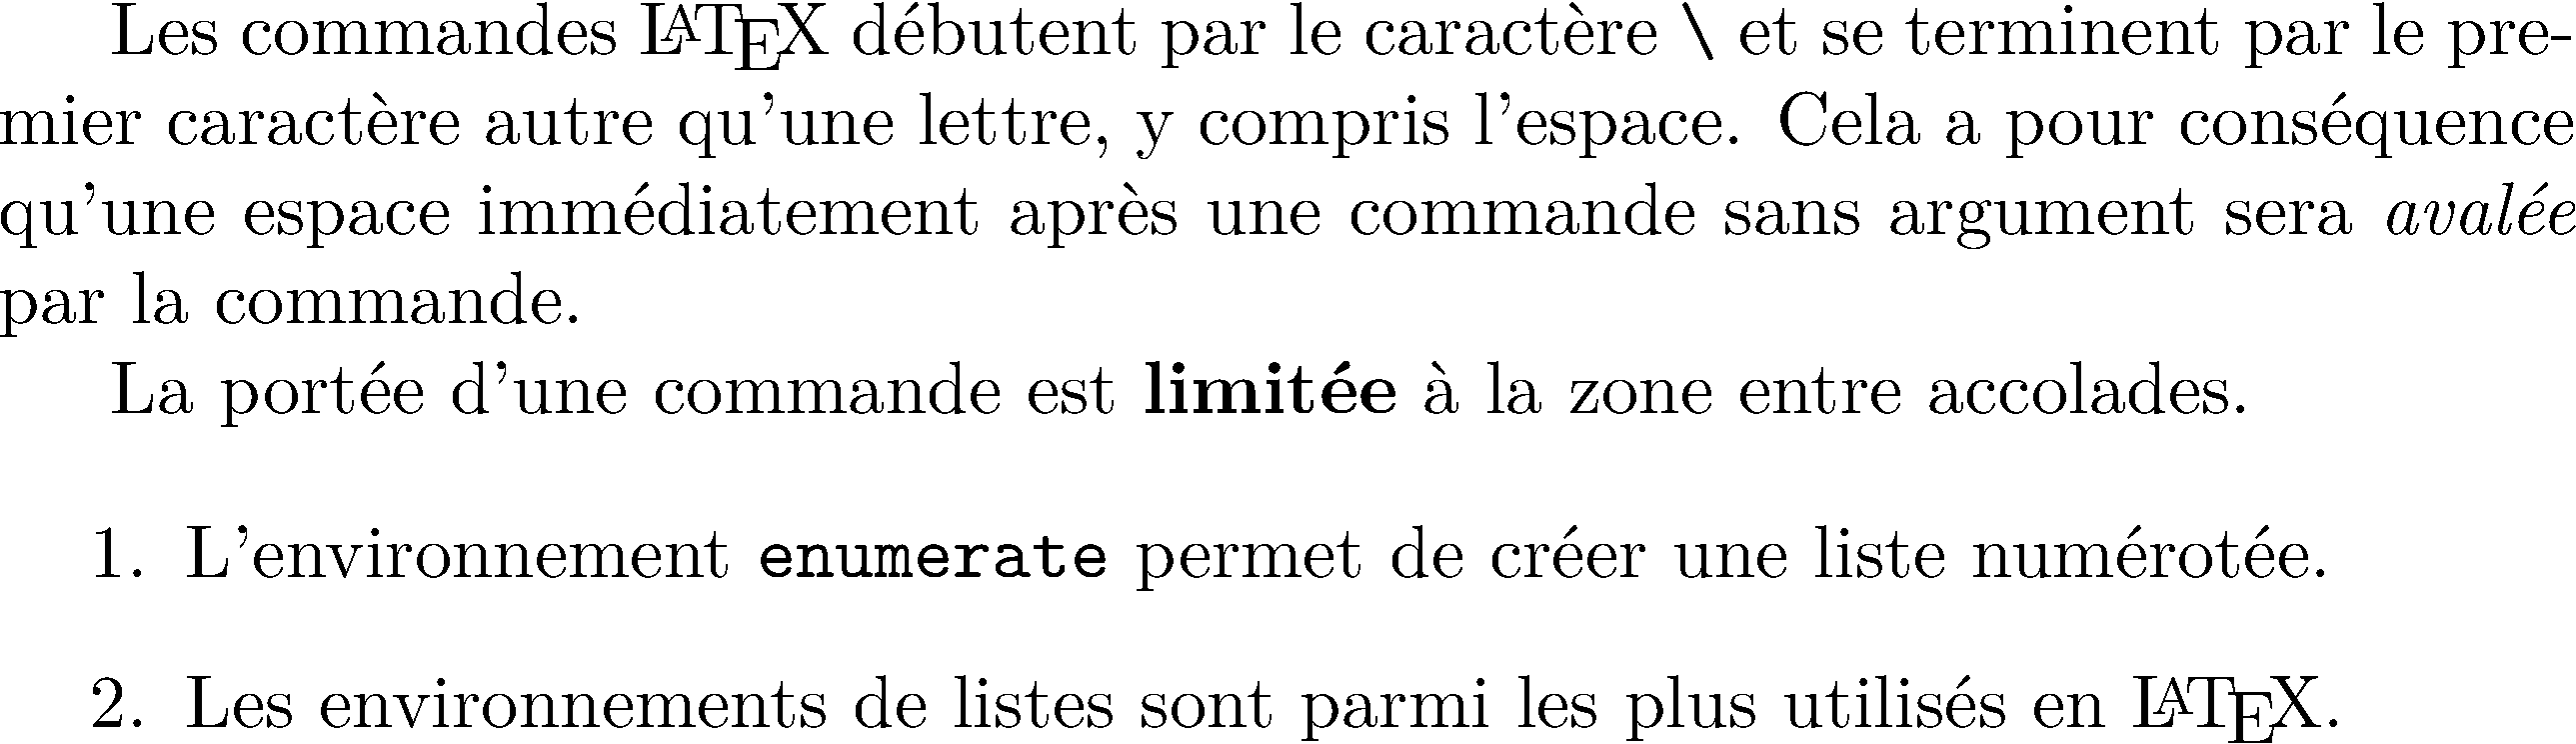
\includegraphics[width=0.95\linewidth]{exercice_commandes-output}
  \end{center}
\end{exercice}

\begin{exercice}[nosol]
  \begin{enumerate}
  \item Compiler tel que fourni le fichier
    \fichier{exercice\_classe+paquetages.tex}.
  \item Changer la police de caractère du document pour 11~points,
    puis 12~points. Changer la classe du document pour \class{memoir}.
    Observer l'effet sur les marges et sur la coupure automatique des
    mots.
  \item Charger le paquetage \pkg{icomma} et observer l'effet sur la
    formule mathématique.
  \item Charger le paquetage \pkg{numprint} avec l'option
    \verb=autolanguage= (\emph{après} le paquetage \pkg{babel}). Dans
    le code source de la formule mathématique, changer
\begin{lstlisting}
10 000
\end{lstlisting}
    pour
\begin{lstlisting}
\nombre{10000}
\end{lstlisting}
    et observer le résultat.
  \end{enumerate}
\end{exercice}


%%% Local Variables:
%%% mode: latex
%%% TeX-engine: xetex
%%% TeX-master: "formation-latex-ul"
%%% coding: utf-8
%%% End:
